\documentclass{article}
\usepackage[utf8]{inputenc}
\usepackage{fullpage}
\usepackage{amsmath}
\usepackage{hyperref}
\usepackage{amssymb}
\usepackage[most]{tcolorbox}
\usepackage{empheq}
\usepackage{mhchem}
\usepackage{braket}
\usepackage{graphicx}
\usepackage{subcaption}

\newtcbox{\mymath}[1][]{%
    nobeforeafter, math upper, tcbox raise base,
    enhanced, colframe=black!30!black,
    colback=black!30, boxrule=1pt,
    #1}
    
\title{Computational Hw 6}
\author{Marcus DuPont}
\date{\today}

\begin{document}

\maketitle

\begin{enumerate}
    \item {\textbf{Newman 10.9}\\
    \begin{figure*}[h!]
    \centering
    \begin{subfigure}[t]{0.5\textwidth}
        \centering
        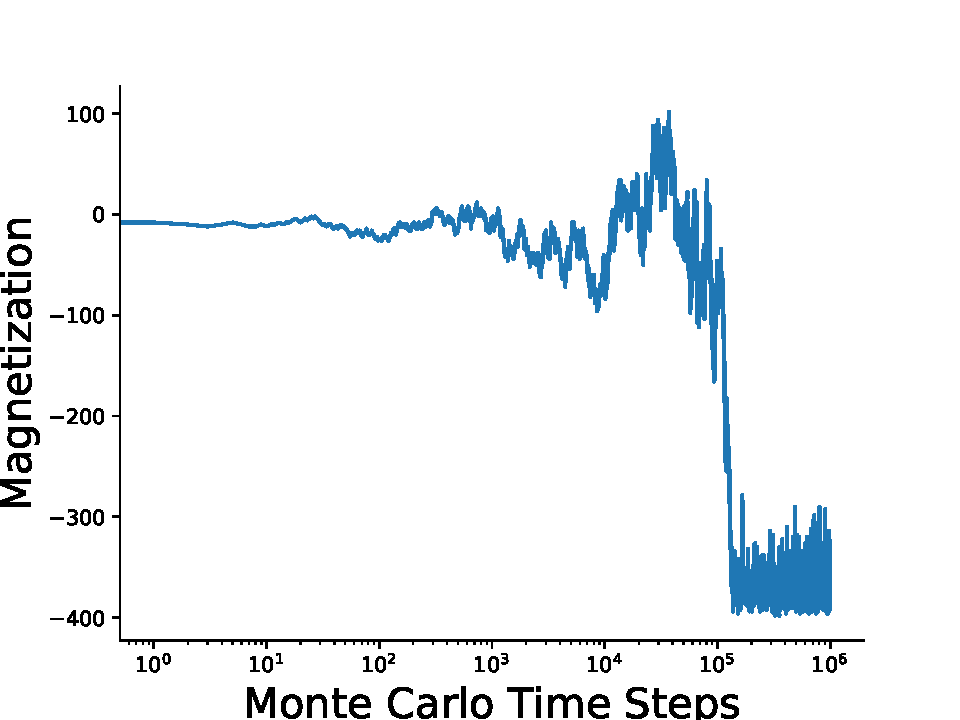
\includegraphics[width=\textwidth, height=10cm]{mplot.pdf}
        \caption{The total magnetization as a function of monte carlo time steps.}
    \end{subfigure}%
    ~ 
    \begin{subfigure}[t]{0.5\textwidth}
        \centering
        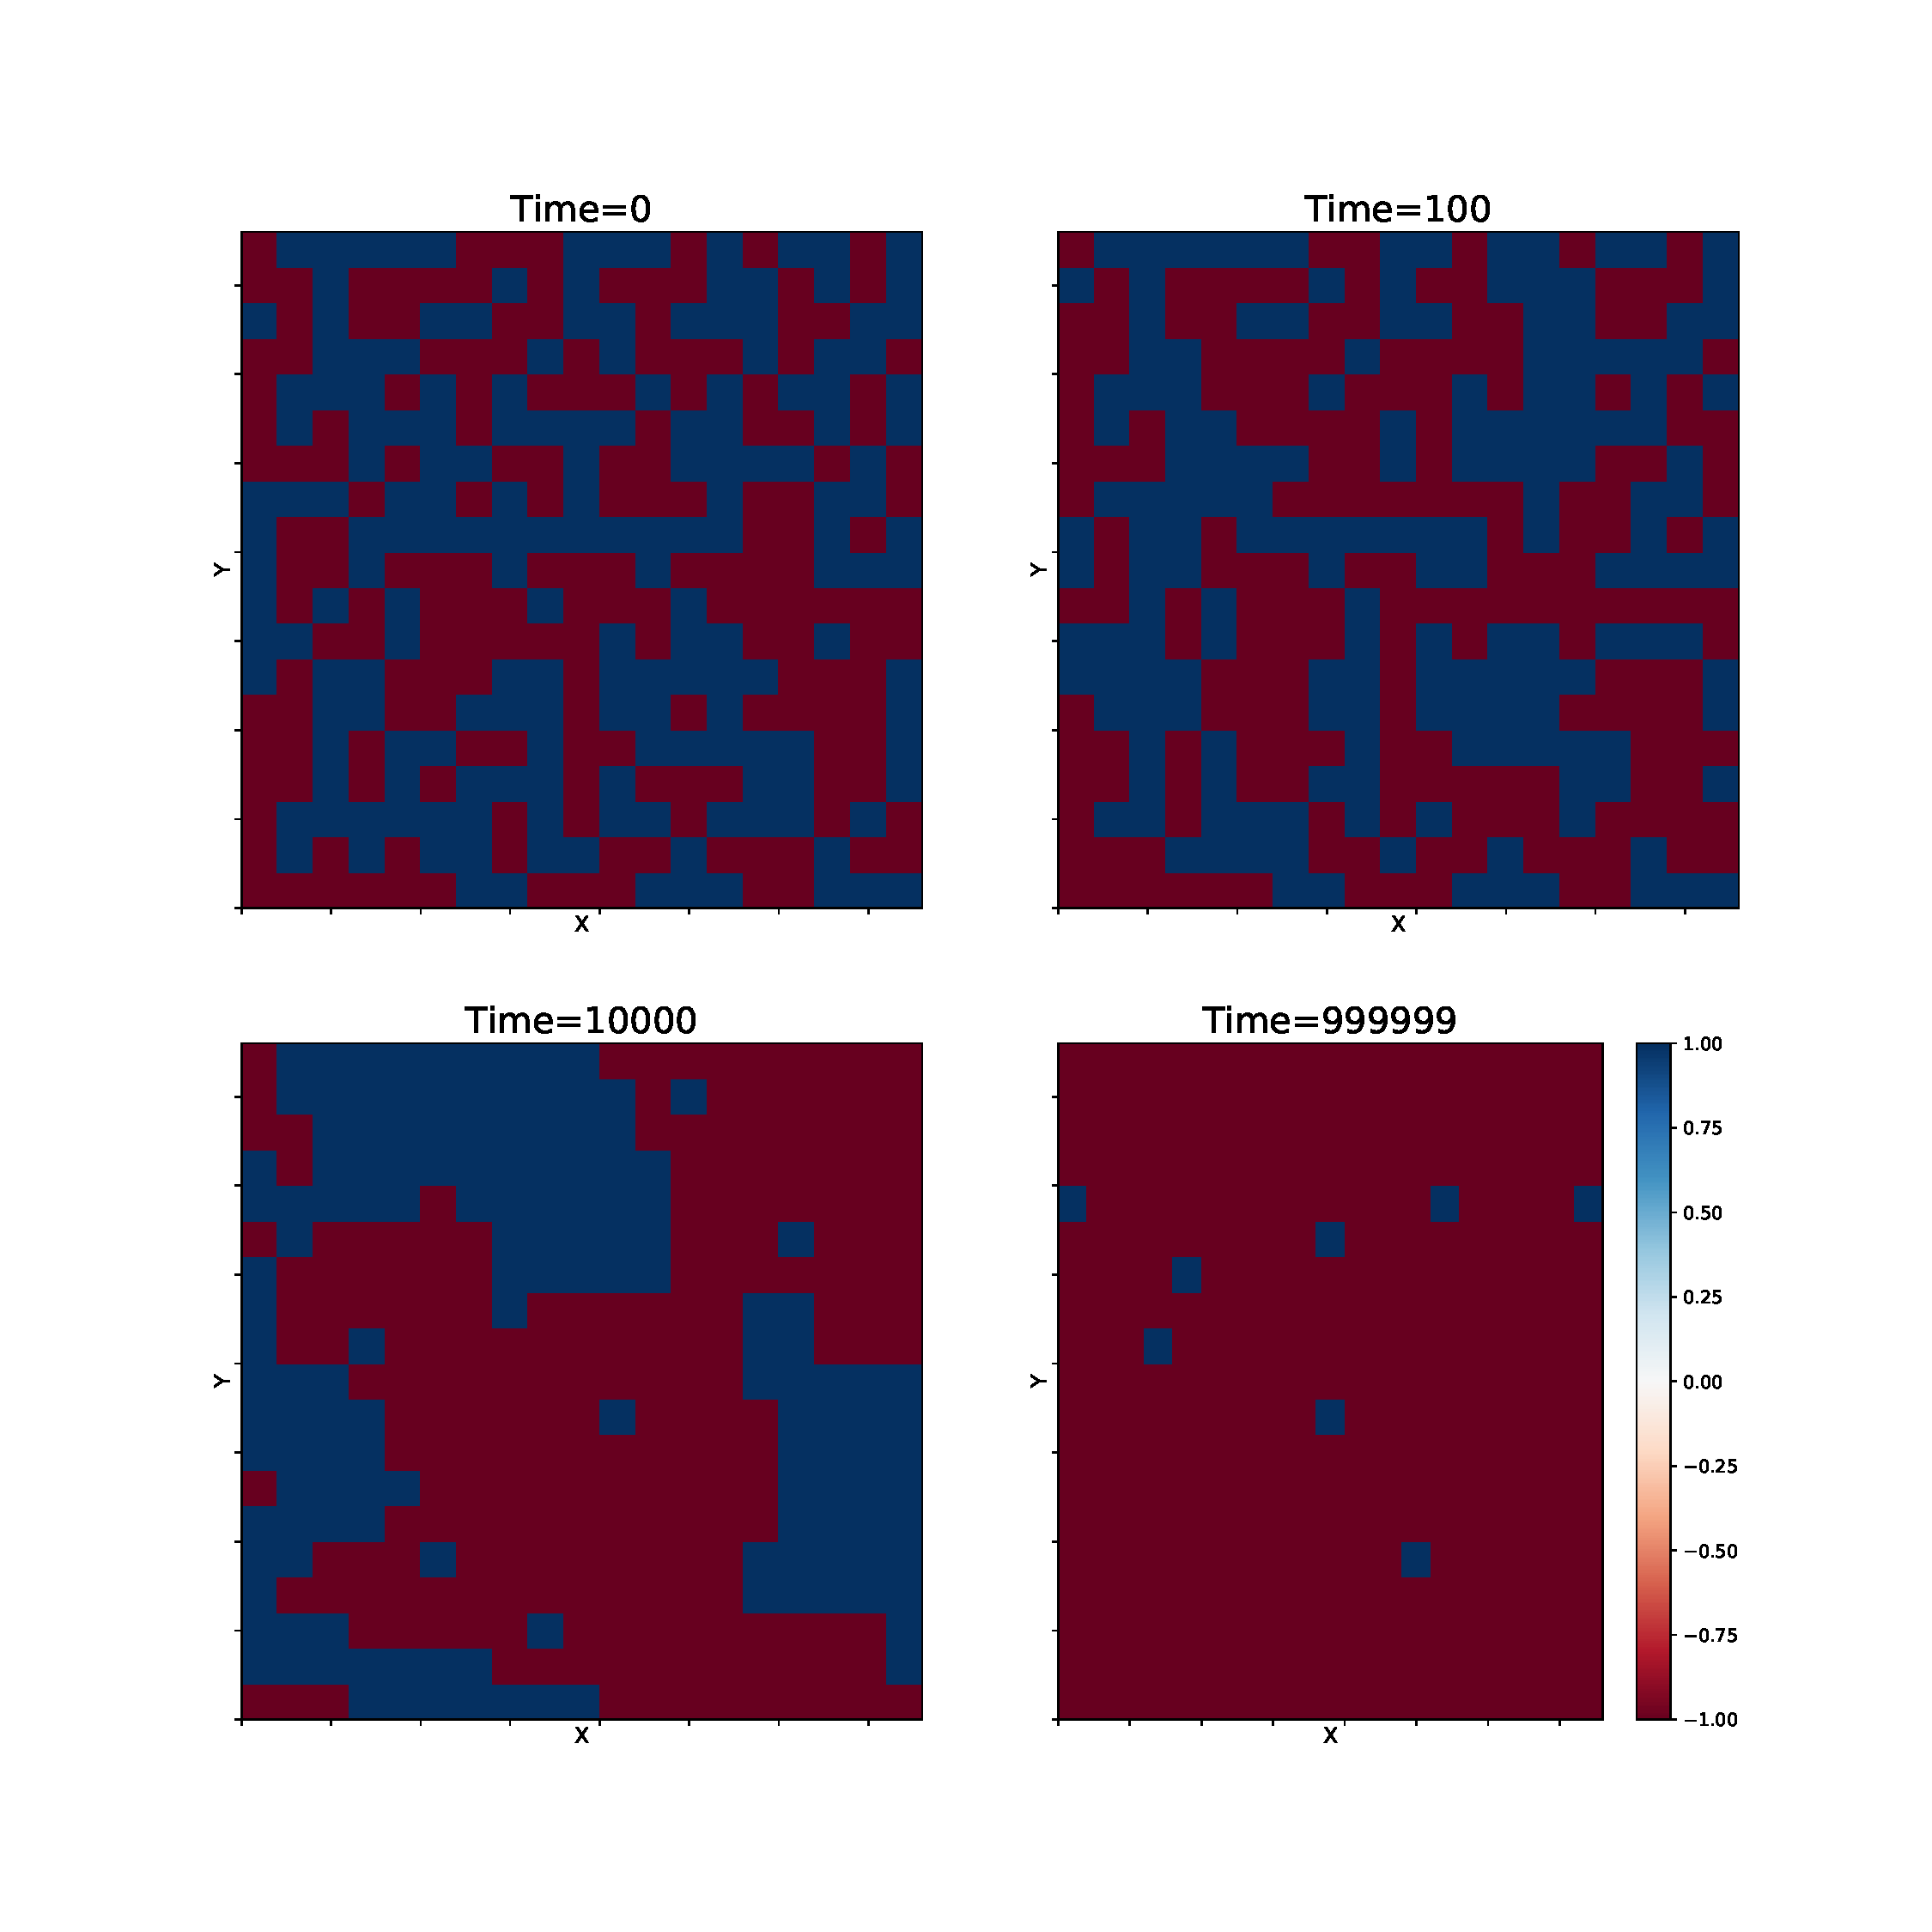
\includegraphics[width=\textwidth, height=10cm]{config.pdf}
        \caption{The magnetic configuration as a function of monte carlo steps}
    \end{subfigure}
    \caption{Example of the behavior of the system configuration as we approach one million steps.}
    \end{figure*}
    The Ising model is a theoretical model of a magnet. Some magnetic material is made up of a bunch of tiny dipoles that prefer to be aligned or anti-aligned depending on the magnetization type. In this model, we explore the \textit{ferromagnetic} properties of some material meaning its overall energy is lower when all of the dipoles are aligned. It is generally assumed that the spins only interact with those immediately adjacent to them (Newman pg. 488) with energy
    \begin{equation}
        E = - J \sum_{\langle ij \rangle}s_is_j,
    \end{equation}
    where $J$ is a positive interaction constant and the notation $\langle ij \rangle$ is indicative of a sum over pairs $i,j$. One way to go about programming this type of model is to take some particle with its respective spin within the lattice and count all of its neighboring interactions. For example,
    \begin{figure*}[h!]
    \centering
    \begin{subfigure}[t]{0.5\textwidth}
        \centering
        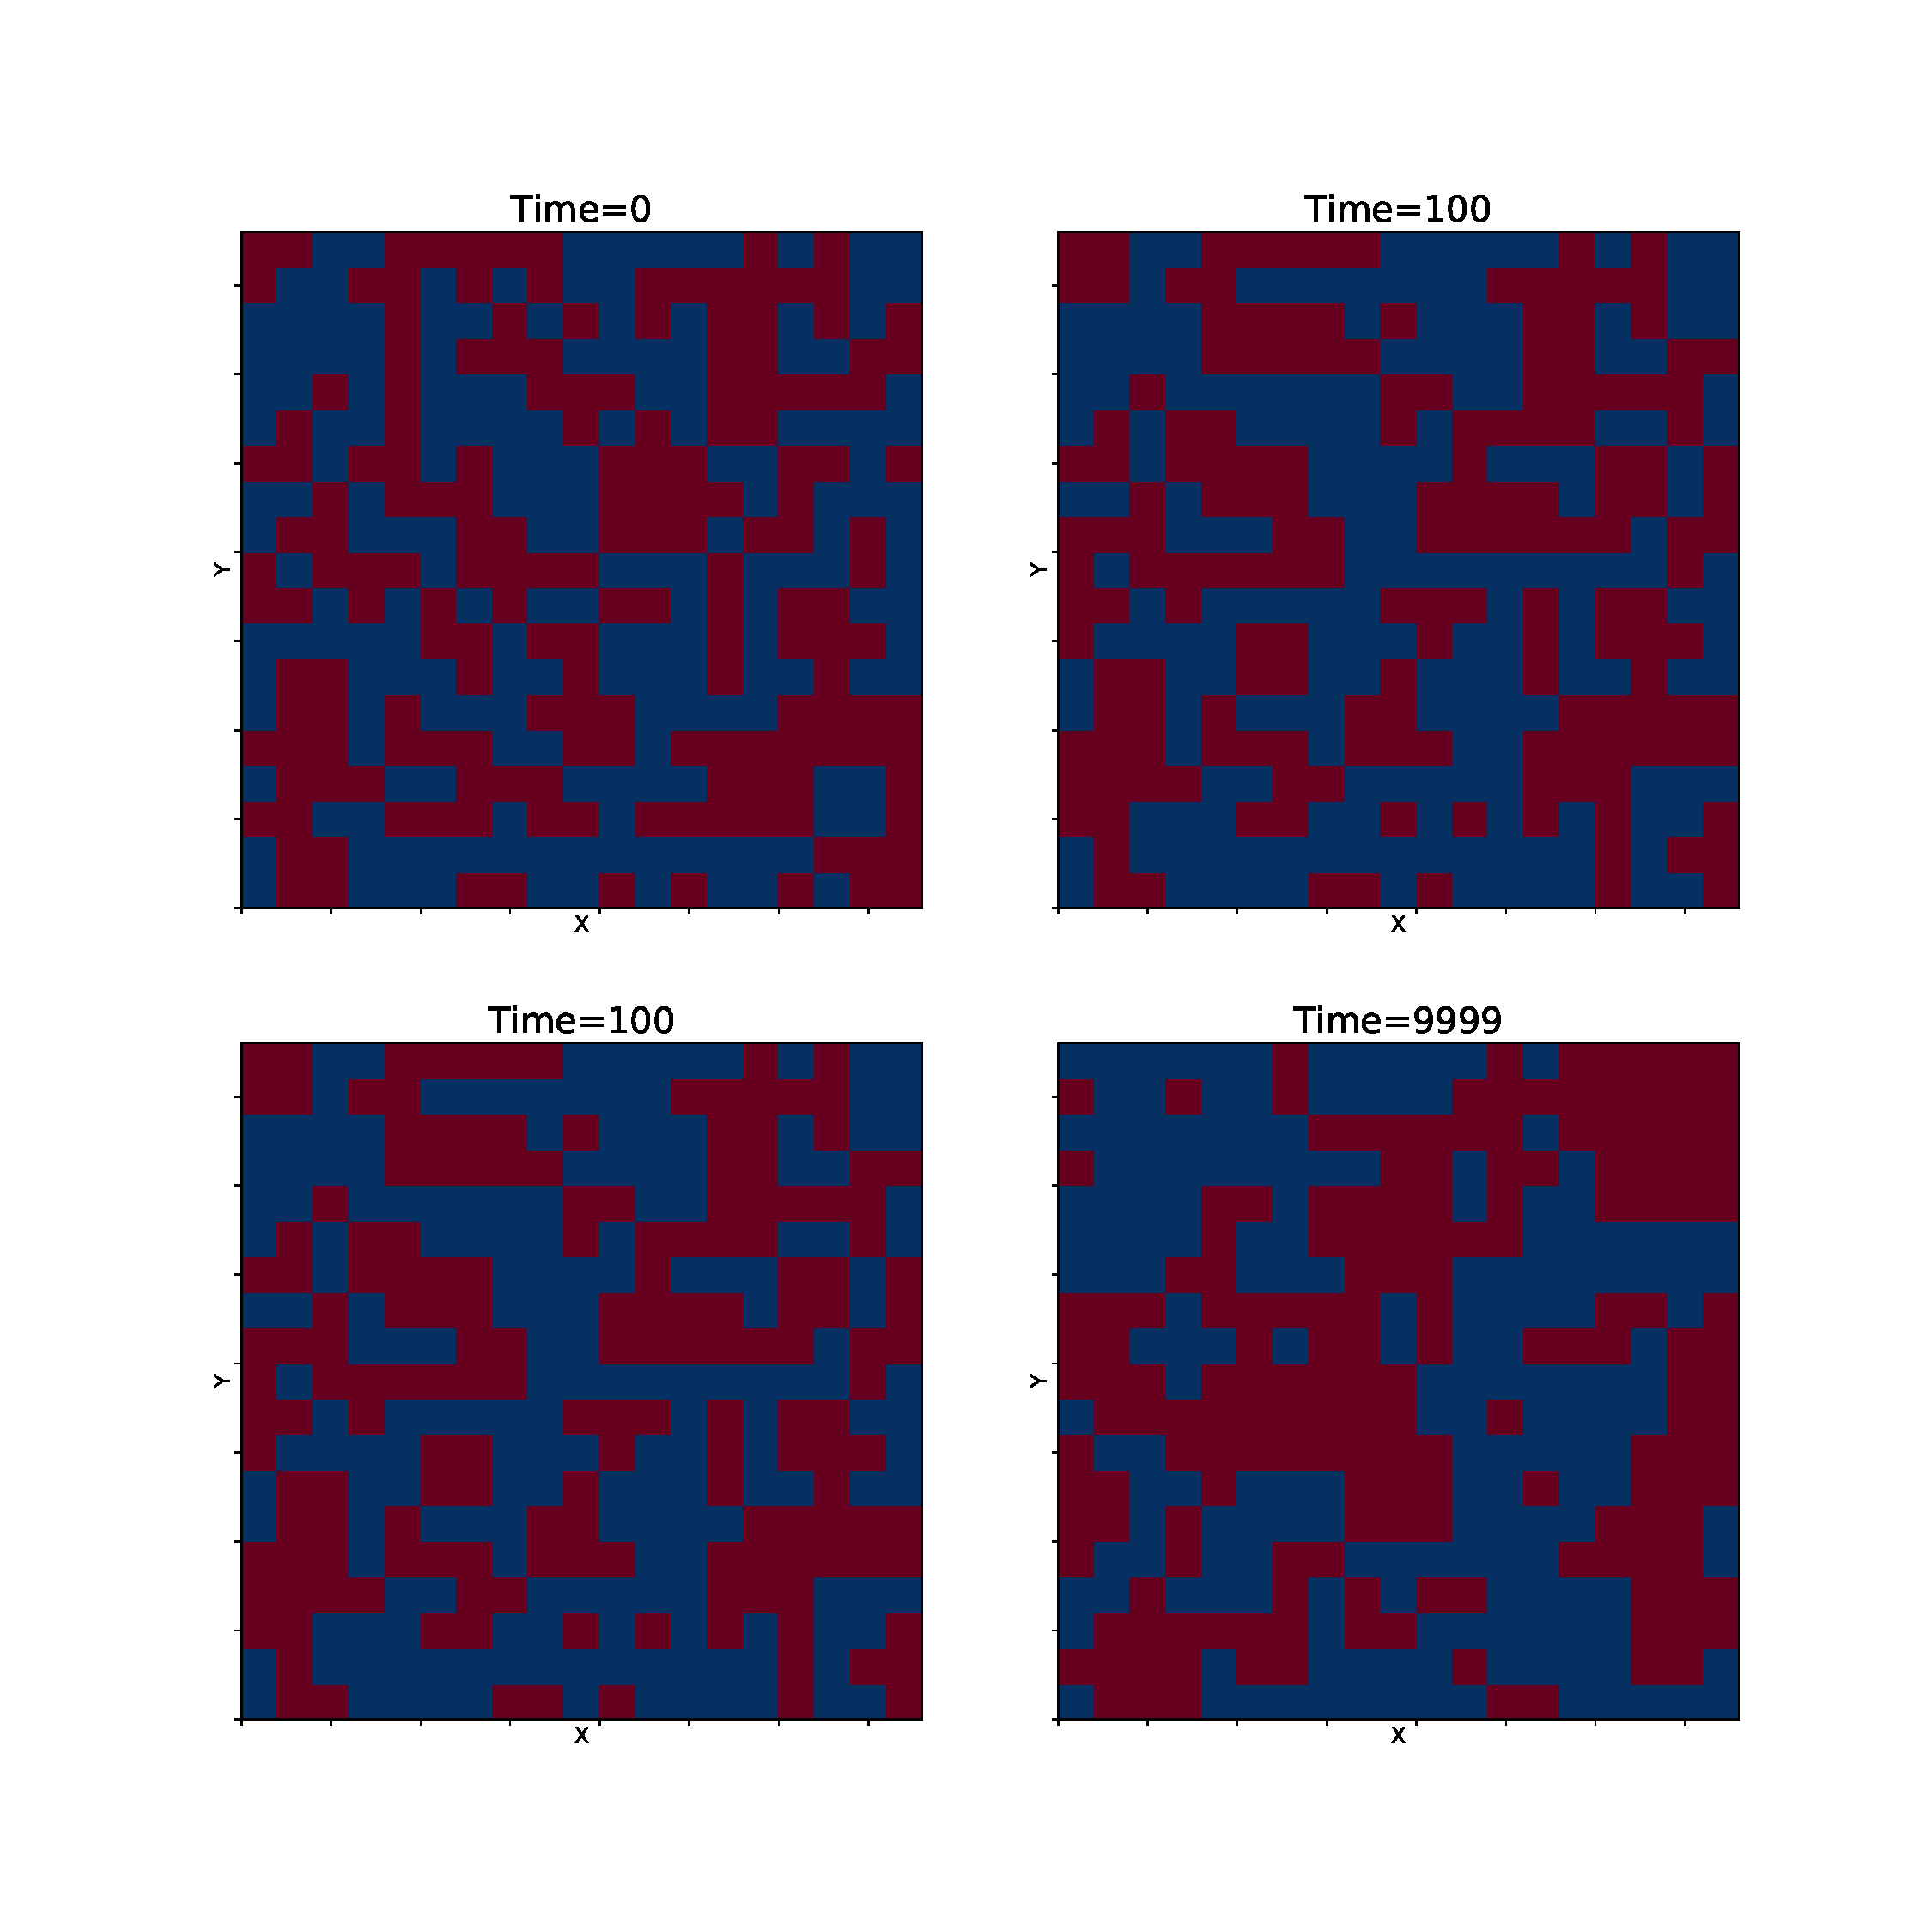
\includegraphics[width=\textwidth, height=10cm]{config2.pdf}
        \caption{The magnetic configuration at $T=2$.}
    \end{subfigure}%
    ~ 
    \begin{subfigure}[t]{0.5\textwidth}
        \centering
        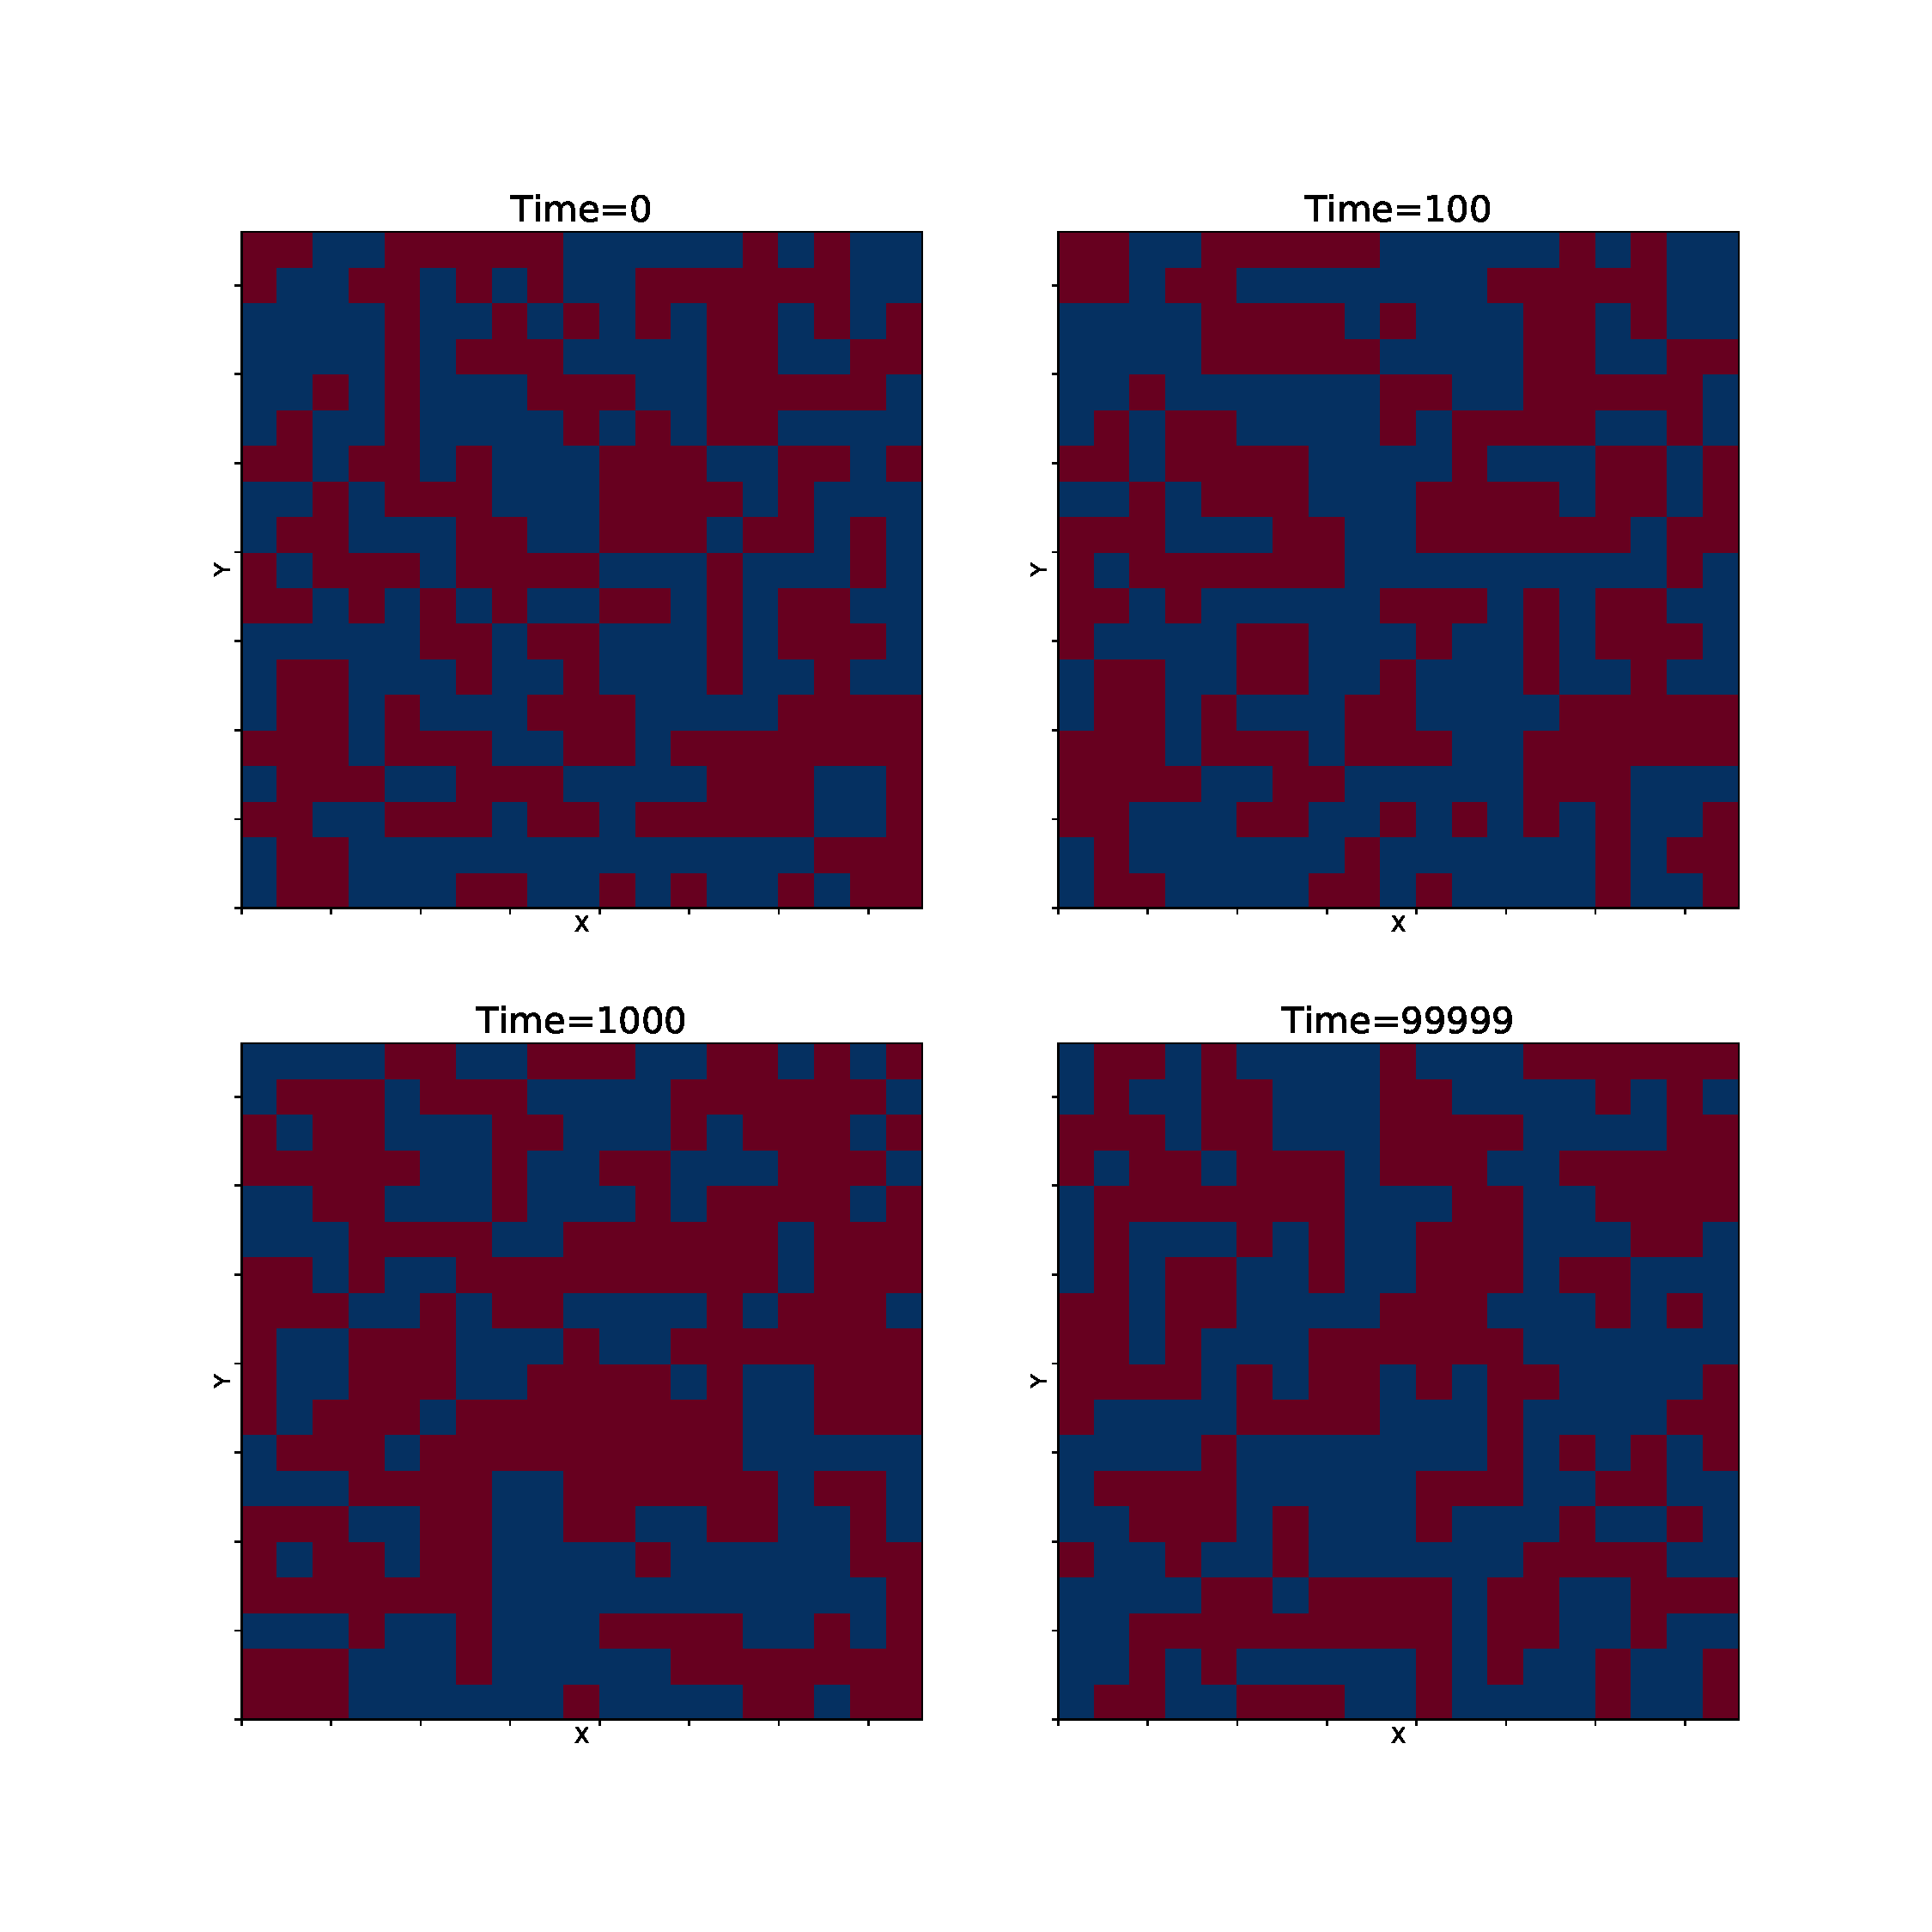
\includegraphics[width=\textwidth, height=10cm]{config3.pdf}
        \caption{The magnetic configuration at a $T=3$.}
    \end{subfigure}
    \caption{An example of the resistance of the material to align if its initial temperature is too high.}
    \end{figure*}
    \begin{align*}
        s &= S_{ij} & \xi = \sum_{i \neq j}S_{ij},
    \end{align*}
    where $\xi$ represents the neighboring atoms (4 in total). The interaction energy is then
    \begin{equation*}
        \begin{split}
            E = -\frac{J}{4}\sum s \xi,
        \end{split}
    \end{equation*}
    where I've divided by 4 to account for the extra counting of the other pairs. With this information we can calculate the total magnetization of the material with the following equation
    \begin{equation}
        M = \sum_i s_i
    \end{equation}
     \begin{figure*}[h!]
    \centering
    \begin{subfigure}[t]{0.3\textwidth}
        \centering
        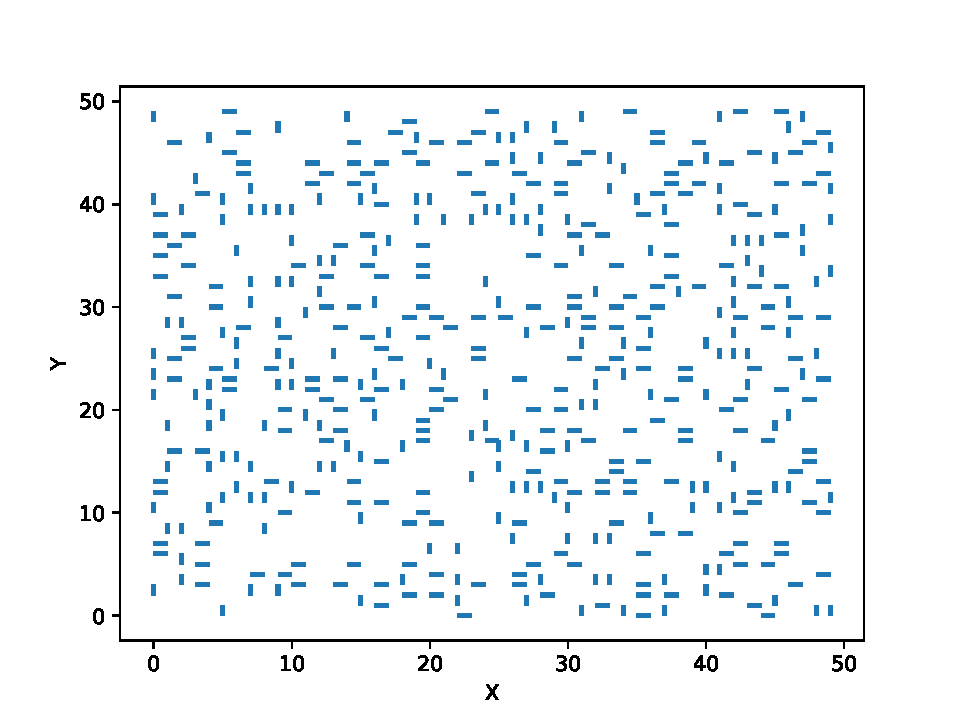
\includegraphics[width=\textwidth, height=7cm]{dimer100.pdf}
        \caption{Dimer density when $\tau = 100$.}
    \end{subfigure}%
    ~ 
    \begin{subfigure}[t]{0.3\textwidth}
        \centering
        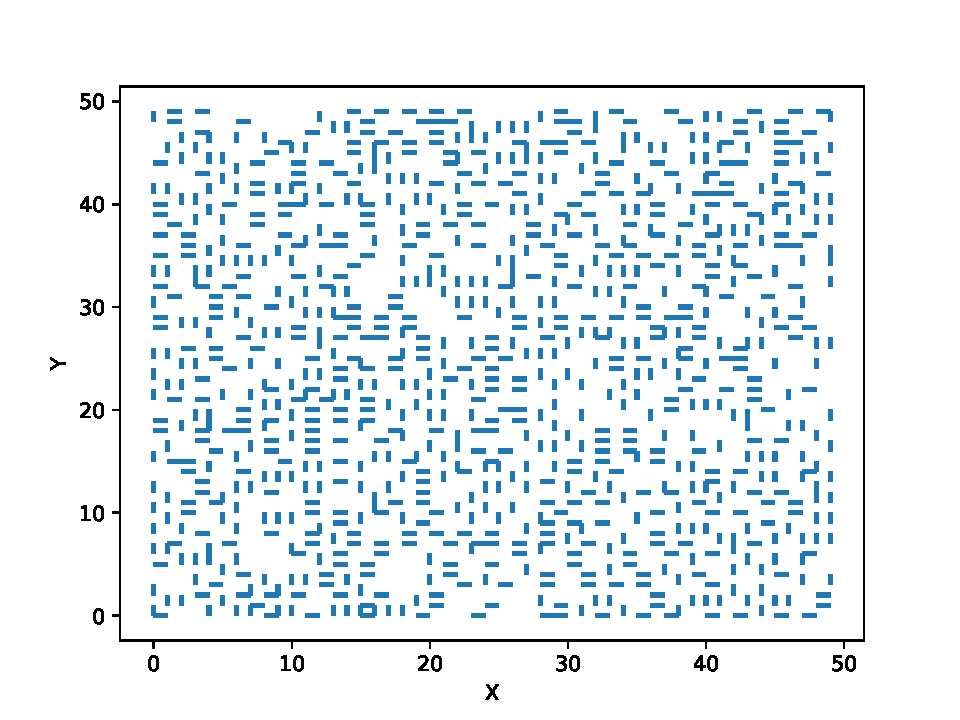
\includegraphics[width =\textwidth, height=7cm]{dimer1000.pdf}
        \caption{Dimer density when $\tau = 1000$.}
    \end{subfigure}
    ~
    \begin{subfigure}[t]{0.3\textwidth}
        \centering
        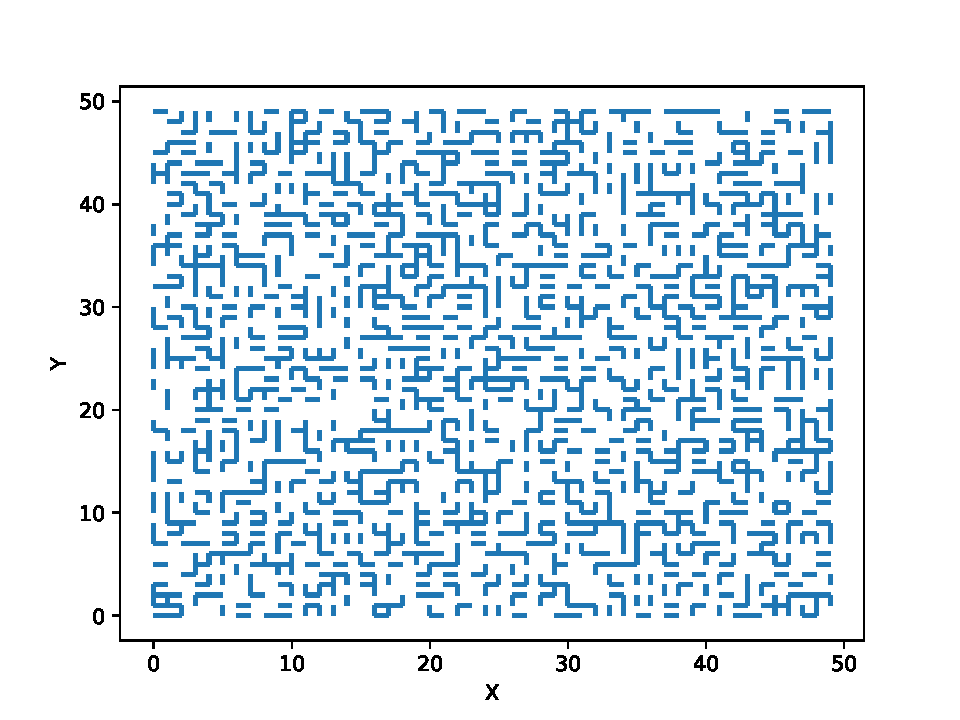
\includegraphics[width=\textwidth, height=7cm]{dimer10000.pdf}
        \caption{Dimer density when $\tau = 10000$.}
    \end{subfigure}
    \caption{The Dimer Density as a function of $\tau$. I recognize that the dimers should not overlap. I spent most of my time trying to fix that issue, but alas...}
    \end{figure*}
    I won't go over the details of utilizing this with the Monte-Carlo Metropolis method for calculating the energy difference when summed over the entire lattice since ore can be read in Mark Newman's book. The results of this method are shown below.
   As we see from the figures, the magnetization timescale increases depending on the total temperature. This is because as a material gets hotter, the kinetic motion of the particles cause them to statistically anti-align. Eventually after some temperature called the Curie Temperature, the total magnetization of the material $\langle M \rangle = 0$.
    }
    \begin{figure}[htp]
        \centering
        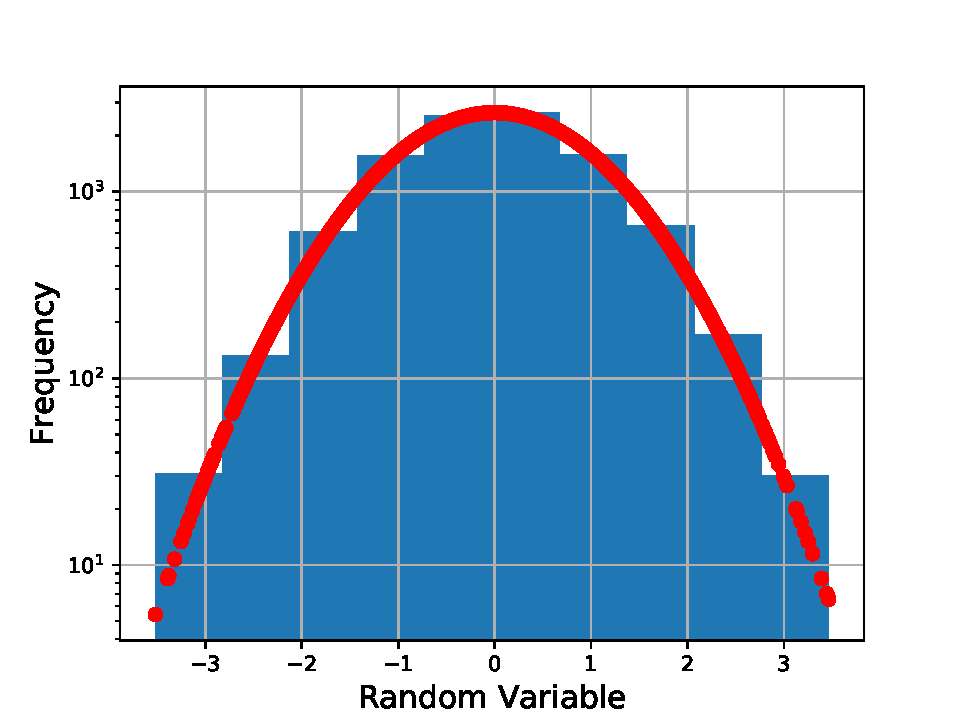
\includegraphics[width=\textwidth, height=9cm]{gaussian_hist.pdf}
        \caption{The distribution of random variable frequencies plotting alongside the normal distribution for comparison.}
        \label{fig:my_label}
    \end{figure}
    \item {\textbf{Newman 10.11}\\
    Dimers are are polymers with two atoms that land on the surface of a solid, sometimes falling in the spaces between the atoms on the surface (Newman pg. 497). These dimers tend to form a grid within the square lattice of the material while they fail to overlap due to Coulomb repulsion. To solve this problem, we use simulated annealing which means that we eventually get the system to converge to a result using thermodynamic concepts. For example, many physical systems can by using a \textit{cooling} schedule of the form
    \begin{equation*}
        T = T_0 \exp(-t/\tau),
    \end{equation*}
    where $T_0$ is the initial maximum temperature and $tau$ is our time constant. Depending on the value of $tau$, certain systems approach the solution at a reasonable time. The results are shown below.
    }
    \item {\textbf{Problem 3}
    Linear Congruential Generators are form of creating what are known as \textit{pseudo} random number generators because they are given in the form
    \begin{equation}
        x' = (a*x +c) \ (\text{mod} \  m),
    \end{equation}
    where $a$ and $c$ are constants and $m$ determines our range or period of random samples. For this task, I used Newman's values for the constants
    
    \begin{align*}
        a &= 1664525 & c &= 1013904225
    \end{align*}
    and I used a periodic value for $m = 2^{32}$. This value was taken from a GNU C library. Next, I created a function that took the parameters in the form $f(n,interval, a, c,m, seed)$ to generate my range of random samples. I then used this random sampler to generate a sequence of Gaussian variables that are derived from the probability distribution
    \begin{equation}
        p(x) = \frac{1}{\sqrt{2\pi \sigma}}\exp\left(\frac{-(x-\mu)^2}{2\sigma^2} \right)
    \end{equation}
    and converted it into
    \begin{equation*}
        r = \sqrt{-2\sigma^2\log(1-z)}
    \end{equation*}
    as described in Newman. A histogram of the randomly generated variables is shown in Figure 2. Once tested for success,
    a power spectrum was calculated for these random variables and is shown in Figure 3. A random walk was then created using the random samples described by the equation
    \begin{equation*}
        x_i = x_{i-1} + b_i,
    \end{equation*}
    where $b_i$ is our i-th Gaussian variable in the sequence. Results of the random walk and power spectrum are shown.
    \begin{figure}
        \centering
        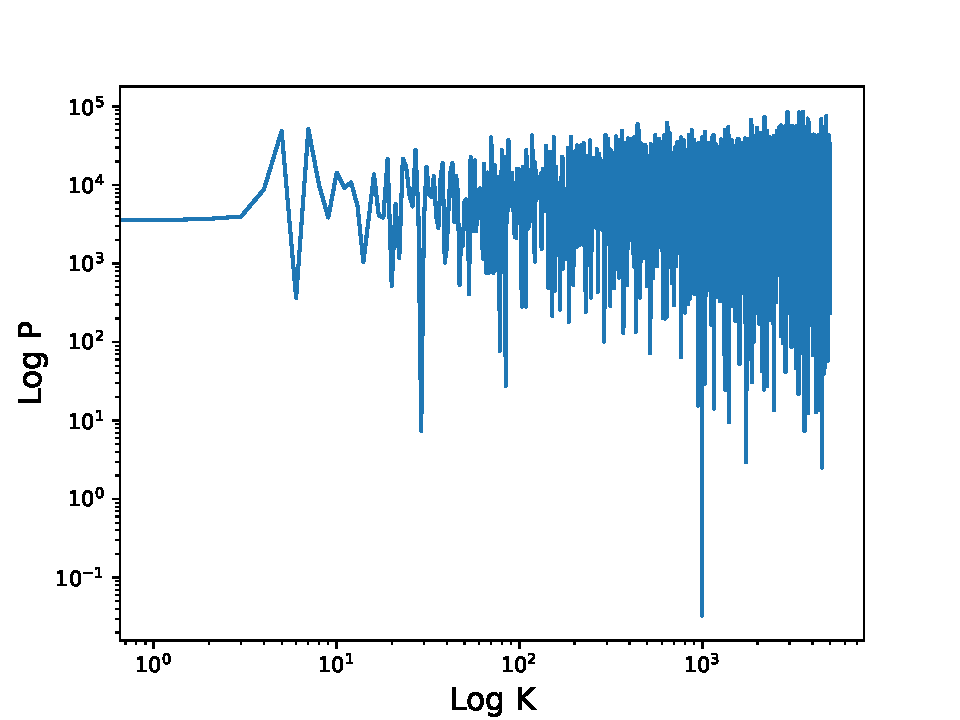
\includegraphics{power_spec.pdf}
        \caption{Power Spectrum of Gaussian Varibales}
        \label{fig:my_label}
    \end{figure}
    \begin{figure}
        \centering
        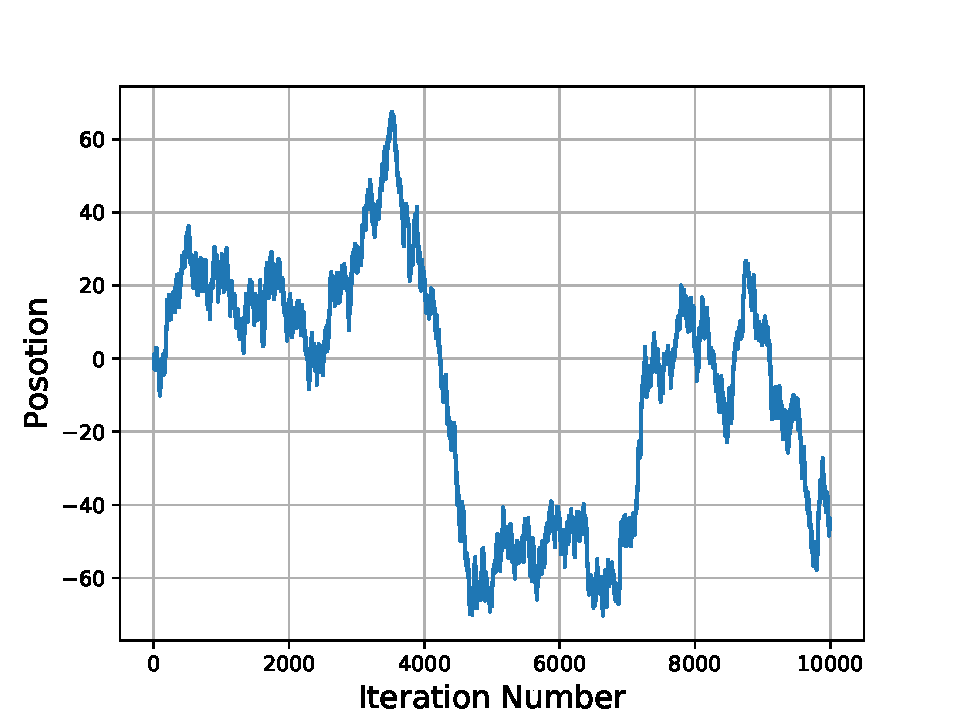
\includegraphics{random_walk.pdf}
        \caption{The random walk generated from the user-created gaussian sample.}
        \label{fig:my_label}
    \end{figure}
    \begin{figure}
        \centering
        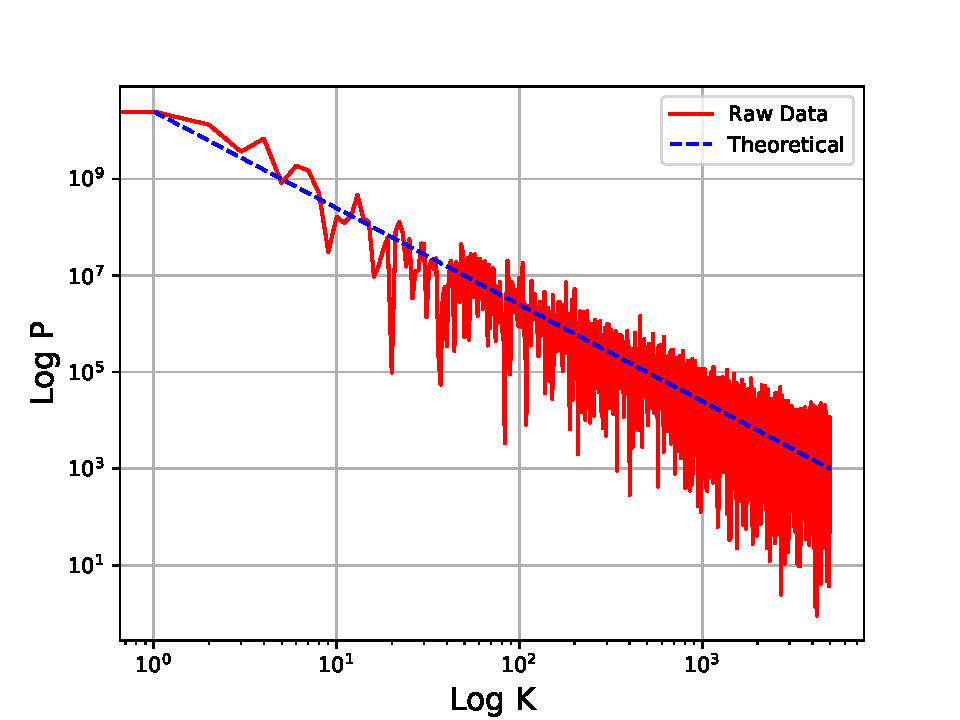
\includegraphics{power_spec_walk.pdf}
        \caption{Power Spectrum of random walk which indeed shows the $P \propto k^{-2}$ relationship.}
        \label{fig:my_label}
    \end{figure}
    }
\end{enumerate}

\end{document}
